%% This is an example first chapter.  You should put chapter/appendix that you
%% write into a separate file, and add a line \include{yourfilename} to
%% main.tex, where `yourfilename.tex' is the name of the chapter/appendix file.
%% You can process specific files by typing their names in at the 
%% \files=
%% prompt when you run the file main.tex through LaTeX.
\chapter{Stereo correspondence}
\section{Overview of correspondence problem}
As described earlier,correspondence problem involves determining point-to-point relationship between 2 views but since these views come from projective elements like cameras,projectors,a pixel-to-pixel relation between this pair(called binocular-pair or stereo-pair) must be determined. In nutshell,establishing correspondence(technically called stereo-correspondence) means to know for a point in 3D world,which pixel in camera \& in projector(or another camera) will see it. Following section gives introduction to the current state-of-art in field of stereo-correspondence.

\section{State-of-art approaches}
To solve shape-acquisition problem following classification has been reported in literature[23][24]:\newline
1.Contact techniques:\newline
\indent   1.1 Non-destructive techniques:\newline
\indent \indent         1.1.1 Coordinate measurement machines\newline
\indent \indent         1.1.2 Jointed arms\newline
\indent   1.2 Destructive techniques:\newline
\indent \indent         1.2.1 Slicing\newline
2 Non-contact techniques:\newline
\indent   2.1 Transmissive techniques:\newline
\indent \indent          2.1.1 Industrial CT\newline
\indent   2.2 Reflective techniques:\newline
\indent \indent         2.2.1 Optical techniques:\newline
\indent \indent \indent                  2.2.1.1 Active techniques:\newline
\indent \indent \indent \indent                 2.2.1.1.1 Active stereo\newline
\indent \indent \indent \indent                 2.2.1.1.2 Imaging radar\newline
\indent \indent \indent \indent                 2.2.1.1.3 Active depth from defocus\newline
\indent \indent \indent                  2.2.1.2 Passive techniques:\newline
\indent \indent \indent \indent                 2.2.1.2.1 Passive stereo\newline
\indent \indent \indent \indent                 2.2.1.2.2 Depth from defocus\newline           
\indent \indent \indent \indent                 2.2.1.2.3 Shape from shading\newline
\indent \indent \indent \indent                 2.2.1.2.4 Shape from silhouette\newline
\indent \indent         2.2.2 Non-optical methods:\newline
\indent \indent \indent                  2.2.2.1 Microwave radar\newline
\indent \indent \indent \indent          2.2.2.2 SONAR\newline

In this work focus is on active stereo approach using structured light technique. So present survey will describe current state-of-art in structured-light techniques. Structured light systems deploy off-the-shelf video cameras \& projectors as their binocular elements. Here a camera pair of passive stereo methods is replaced by a camera-projector pair. It provides solution to the problem of correspondence for texture-less surfaces experienced by passive stereo camera pair because of lack of texture marks which act as important cues for establishing correspondence. Projection of explicit patterns which create an artificial texture on object surface,greatly simplifies the problem of correspondence. In these techniques,projector projects a pattern(s) which encode the information regarding the projector pixel which has illuminated a point in the scene. Camera captures these patterns and by decoding the pattern which is functionally equivalent to solving the correspondence problem in passive stereo vision,it extracts the unique ID of projector pixel that illuminated the same point in 3D space as is captured by camera. Figure~\ref{fig:sls}\footnote{Figure source: Refer~\cite{25}} provides conceptual representation of structured-light systems.\newline

\begin{figure}[hb]
\centering
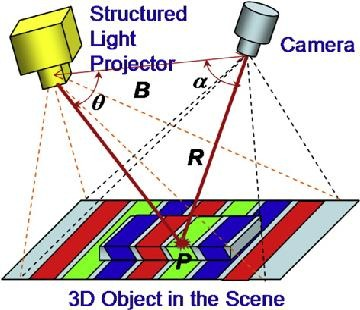
\includegraphics[width=7cm,height=7cm]{../img_source/struct_light.jpg}
\caption{A typical structured light system}
\label{fig:sls}
\end{figure}

\noindent
In figure~\ref{fig:sls},$\theta$  denotes the angle between a projector optical-ray \& baseline between camera and projector optical center.Similarly $\alpha$ denotes the angle between corresponding camera optical-ray \& baseline between camera and projector optical center.Projected pattern in the figure is just a representative of structured-light technique.\newline
\noindent
Structured light techniques have been classified in 4 major classes[23][24][26] based on how correspondence information is encoded in the projected patterns:
\paragraph{Time multiplexing.}Every point is encoded by series of intensities across multiple patterns.
\paragraph{Spatial encoding.}Every pixel is encoded based on intensities of its neighborhood pixels. 
\paragraph{Direct encoding.}Every pixel is encoded by its unique intensity and does not depend upon any spatial or temporal correlations among pixels.
\paragraph{Hybrid encoding.}It encodes pixels both spatially and temporally to project  lesser number of patterns than conventional time-multiplexing techniques and to have more robustness as compared to spatial methods.\newline \newline
\noindent
It should be noted however that this classification do not enforce unique code for each projected pixel i.e., there may be a set of pixels with same code. This pattern design decision depends upon required resolution in the reconstructed scene.

\begin{enumerate}
\item \textbf{Time multiplexing}\newline    
\noindent 
Time multiplexing techniques encode unique ID's for pixel(s) of projector over multiple patterns projected sequentially over a period of time. Camera captures all these pattern in an order to determine correct ID for each pixel(or pixel group). Depending upon type of correspondence required i.e. camera-pixel to projector-pixel or camera pixel-plane to projector pixel-number of axes of codification can be chosen to be both vertical and horizontal or one of them respectively. To be more clear, axis of codification means axis of projected pattern along which the codes are embedded other axis will simply have same copy of intensity for each code in each pattern and hence will not contribute to pixel codification. Examples of time-multiplexing based structured light patterns are binary-coded patterns, N-ary codes, gray code+phase shift method. Here i will discuss these methods as representatives for time multiplexing approach.
\begin{enumerate}
\item \textbf{Binary coded patterns} \newline
\noindent
In these patterns[27], any pixel in camera and projector is identified by the sequence of binary intensities it receives or projects respectively. Specifically, for a $N*M$ projector resolution, if pixels are to be divided into K groups along say Horizontal axis then a total of $\frac{N}{K}$ code-words will be used which will requires projection of $\log_2\lceil\frac{N}{K}\rceil$ patterns sequentially. A pattern say $j^{th}$ will represent intensities corresponding to the $j^{th}$ bit of all code-words across its horizontal axis. Hence every pattern is called a \textit{bit-plane}. Figure~\ref{fig:bin_pattern_design}\footnote{Figure source: Refer~\cite{25}} shows design of code-words, figure~\ref{fig:bin_pattern_project}\footnote{Figure source: Refer~\cite{25}} shows projection of simple binary-coded patterns scheme.After all patterns are captured by camera, a code at every pixel is computed based on intensities incident on that pixel during pattern projection. A single pattern determines single bit in code-word of all pixels in the camera image.
  

\begin{figure}
\centering
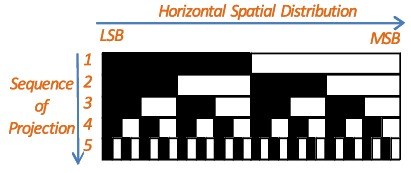
\includegraphics[width=8cm,height=5cm]{../img_source/coded_pattern_design.jpg}
\caption{Binary coded pattern:Design}
\label{fig:bin_pattern_design}
\end{figure}

\begin{figure}
\centering
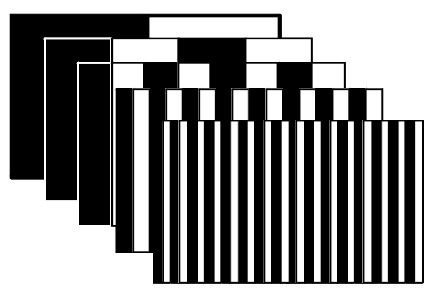
\includegraphics[width=8cm,height=5cm]{../img_source/coded_pattern_projection.jpg}
\caption{Binary coded pattern:Projection}
\label{fig:bin_pattern_project}
\end{figure}



\item \textbf{N-ary coded patterns}\newline
\noindent
In case of binary-coded patterns it can be observed that for high resolution more code-words will be required which directly increases the number of patterns to be projected. For applications requiring faster acquisition rates, number of patterns can be reduced yet meeting the resolution requirement if we increase number of intensity levels that a pixel can have[25][28][29]. This approach can allow for dynamic scene shape recovery at the cost of decreased robustness against environmental noise. As it can be deduced, color-coded patterns are special cases of this technique. Figure~\ref{fig:gray_pattern}\footnote{Figure source: Refer~\cite{25}} shows the gray-level coding scheme, here multiple allowed gray-level can be observed.

\begin{figure}[ht]
\centering
\def\tabularxcolumn#1{m{#1}}
\begin{tabularx}{\linewidth}{@{}cXX@{}}
\begin{tabular}{c c c}
\hspace{2.5cm}
\subfloat[]{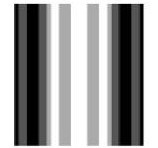
\includegraphics[width=3cm,height=3cm]{../img_source/gray_code_1.jpg}} &
\subfloat[]{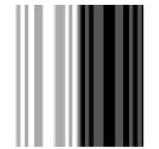
\includegraphics[width=3cm,height=3cm]{../img_source/gray_code_2.jpg}} &
\subfloat[]{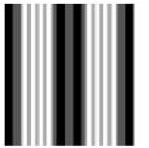
\includegraphics[width=3cm,height=3cm]{../img_source/gray_code_3.jpg}} \\
\end{tabular}
\end{tabularx}
\caption{Gray coded patterns}
\label{fig:gray_pattern}
\end{figure}

\item \textbf{Combination of gray-coded patterns and phase-shift techniques}\newline
\noindent
Gray-coded patterns were proposed to increase robustness of code recovery process against possibility of false-code extraction as compared to simple binary-coded patterns, since successive gray code-words differ at only one bit position thereby reducing chances of assigning same code to the pixels belonging to neighboring code-word groups. It has a straightforward analogy with the considerations in code designing for noisy communication channel. For a treatment of structured-light patterns in way similar to communication code designing over a noisy channel, refer[30].\newline


In phase-shift technique, phase shifted sinusoidal interference fringes are projected on object surface. In camera, unique code to each pixel is assigned in the form of phase of the signal incident on it. Similarly in projector image a phase value is assigned to each pixel which represents spatial position of that pixel in the projected sinusoidal periodic waveform. It can be deduced that this phase value indirectly encodes the position of projector pixel that projected that signal and hence the correspondence information. Figure~\ref{fig:phase_gray_method}\footnote{Figure source: Refer~\cite{25}} shows the spatially aligned combination of phase-shifted and gray coded patterns. Further details of this technique are described in section-3.4 with its actual working.\newline


Gray-coded patterns provide a way to determine a region of pixels uniquely by assigning unique code to it, whereas phase-shift technique can provide phase variation up to pixel-level within that region. Although phase-shift technique is potent to be used alone to provide pixel-level resolution but computational complexity of accurate phase value computation constraints the image resolution and scene geometry.[31] describes details of problems in accurate phase estimation called \textit{phase-unwrapping}. Hence to alleviate problem of low resolution of gray-coded patterns and computationally expensive phase-unwrapping problem, combination of both techniques is used. Here period number of a sinusoidal fringe is determined with the help of gray-coded pattern and pixel-level correspondence within that period is computed using phase-shift technique. Although it comes at a cost of increased number of patterns(typically greater than 10) that must be projected as compared to the original phase shift approach which typically requires 3 or 4 patterns. In pattern design, width of a code-word(in pixels) is equal to width of a period in phase-shifted pattern to assign a unique code-word to each fringe period and hence perform phase unwrapping. A variant of this approach is the subject of this work.

\begin{figure}[!h]
\centering
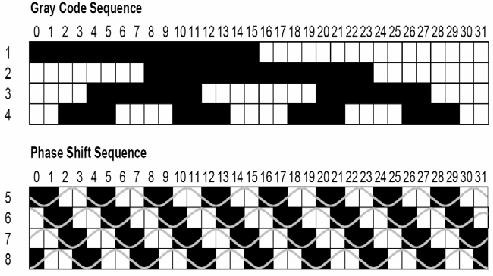
\includegraphics[width=15cm,height=8cm]{../img_source/gray+phase.jpg}
\caption{Combination of Phase-shift and gray code techniques}
\label{fig:phase_gray_method}
\end{figure}
\end{enumerate}
\item \textbf{Spatial encoding methods}\newline
As already mentioned these methods extract more information per pattern by encoding unique identity of pixels in their neighborhood(called \textit{window}) also. Although it can be clearly argued that this approach will have less robustness as compared to time-multiplexing methods since error in a decoding of one pixel will affect decoding of all dependent pixels. Here size of the window is directly proportional to the number of pixels encoded and inversely proportional to the number of intensity levels used for encoding. Basically, aim of these methods is to obtain correspondence from single captured image which facilitates them to be used for dynamic scenes(like moving objects). As can be noticed, increased number of allowed intensity-levels increases chances of error in decoding because natural scene illumination can potentially interact with these projected patterns making accurate pattern decoding more challenging than binary-coded patterns. De Bruijn patterns and M-arrays are discussed here as representatives of this technique.

\begin{enumerate}
\item \textbf{De Bruijn sequence based pattern}\newline
\noindent
De Bruijn sequence[32] of order 'm' over an alphabet of 'n' symbols is a pseudo-random sequence of length $n^m$ where every possible combination of length 'm' occurs only once. These sequences have been adapted for pattern generation by considering number of allowed intensity-level as 'n' and window length as 'm'. In terminology of graph theory it can be interpreted as a graph of $n^m$ vertices and problem of generating debruijn sequence is to determine a Hamiltonian path in that graph, this problem is also called Traveling salesmen problem. Specifically, a pattern encodes a debruijn sequence. Pattern is divided into slits where each slit has width equal to the order of the pattern. Intensities of sub-slits are generated using individual code-words occurring in debruijn sequence. Total number of intensity levels used in the pattern are limited by the alphabet size of used de-bruijn sequence. To decode a pixel it is only required to determine the code-word or window to which it belongs which will depend upon the intensities of its neighborhood pixels. Figure~\ref{fig:de_bruijn}\footnote{Figure source:~\cite{33}} shows patterns generated using debruijn sequence of various alphabets and order. 


\begin{figure}[ht]
\def\tabularxcolumn#1{m{#1}}
\begin{tabularx}{\linewidth}{@{}cXX@{}}
\begin{tabular}{lr}
\subfloat[alphabet:4,order:3]{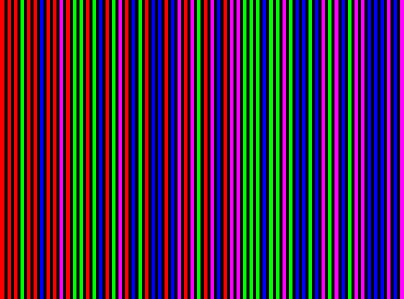
\includegraphics[width=8cm,height=3cm]{../img_source/de_bruijn_1.jpg}} &
\subfloat[alphabet:4,order:3]{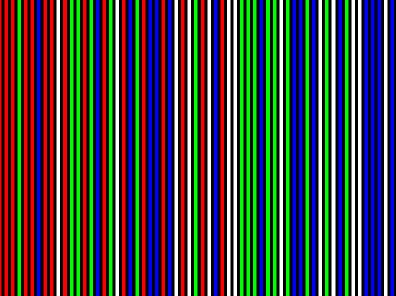
\includegraphics[width=8cm,height=3cm]{../img_source/de_bruijn_2.jpg}} \\
\subfloat[alphabet:3,order:4]{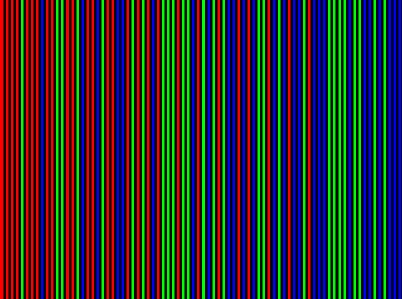
\includegraphics[width=8cm,height=3cm]{../img_source/de_bruijn_3.jpg}} &
\subfloat[alphabet:4,order:4]{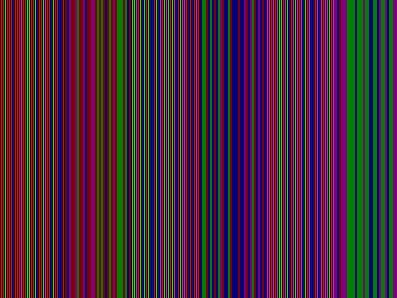
\includegraphics[width=8cm,height=3cm]{../img_source/de_bruijn_4.jpg}} \\
\end{tabular}
\end{tabularx}
\caption{De-bruijn sequence patterns}
\label{fig:de_bruijn}
\end{figure}


\item \textbf{M-array based pattern}\newline
\noindent
M-arrays[34][35] are bi-dimensional extensions of debruijn sequences. Hence a M-array of $N*M$ dimension will have all 2D code-words(in window) of dimension $W*H$ that will occur only once in complete sequence/array. One code-word will be present in one window,so it precisely means that one 2D-window will appear only once in the whole array. Figure~\ref{fig:m_array} shows a M-array based pattern.

\begin{figure}[h!]
\centering
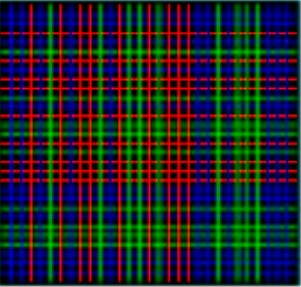
\includegraphics[width=5cm,height=5cm]{../img_source/m_array.jpg}
\caption{M-array based pattern}
\label{fig:m_array}
\end{figure}
\end{enumerate}

\item \textbf{Direct coding techniques}\newline
\noindent
In these techniques, every encoded pixel is identified by its own color/intensity. Although theoretically high resolution for dynamic scenes can be attained but practically these approach are highly susceptible to noise because of large number of intensity-levels used. It also implies that camera with very large pixel depth have to be used for detecting changes in intensity across the scene to extract code from it. Efforts in this direction include grey patterns[36][37][38] for example intensity ratio based grey pattern by [36] which fades away from black to white. Colored patterns[39][40] for example [39] proposed projection of rainbow pattern whereas [40] proposed relatively robust patterns which effectively cancels out the object color by projection of three shifted patterns but at the cost of increasing acquisition time. This approach can be classified as hybrid approach also since it includes combination of direct and temporal techniques. Figure~\ref{fig:rainbow}\footnote{Figure source: Refer~\cite{26}} shows the 3 shifted rainbow pattern as representatives of colored patterns used for direct coding techniques.

\begin{figure}[ht]
\def\tabularxcolumn#1{m{#1}}
\begin{tabularx}{\linewidth}{@{}cXX@{}}
\begin{tabular}{c c c}
\subfloat[]{
\includegraphics[width=5cm,height=5cm]{../img_source/rainbow_1.jpg}} &
\subfloat[]{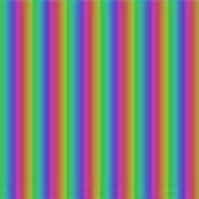
\includegraphics[width=5cm,height=5cm]{../img_source/rainbow_2.jpg}} &
\subfloat[]{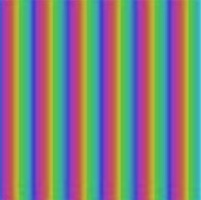
\includegraphics[width=5cm,height=5cm]{../img_source/rainbow_3.jpg}} \\
\end{tabular}
\end{tabularx}
\caption{Direct coding method:Rainbow patterns}
\label{fig:rainbow}
\end{figure}
\vspace{1.5cm}
\item \textbf{Hybrid coding techniques}\newline
\noindent
In order to attain benefits of both spatial and temporal techniques, hybrid patterns[41] were also proposed where patterns are projected temporally but their encoding also depends on neighborhood thereby allowing more information to be encoded per pattern and increased robustness from temporal technique since multiple frames contain the encoding information hence dependence on neighborhood pixels is less as compared to purely spatial neighborhood approach. This approach allowed for slow motion in the scene which is exceptional from point of view temporal-encoding schemes.
\end{enumerate}

\section{Approach followed in this work}
In this work, i have attempted to investigate the accuracy achievable by Phase-shift technique for 3D scanning since currently it is the most popular approach[42][43] for its claimed capability to achieve high accuracy and resolution in the structured-light category. It was decided to develop it also rather than just accuracy analysis because there is no \textit{open-source} implementation available for this technique except the work of [44] but it does not have documentation, is still under development and it is only for windows platform whereas we are working mainly on Linux systems. Work by [45] also attempted for three phase scanning but at the time of development had no means for system calibration and had only naive phase unwrapping algorithm which was far from being usable as a reference for accuracy analysis. \newline


Here, a combination of phase-shift technique with binary coded patterns instead of purely using phase-shifting based approach is used, reason for which is described in section-3.5. This approach gives higher spatial resolution of phase-shift technique and high noise robustness and considerable reduction in correspondence computation complexity of binary-coded patterns. Implementation details of this approach will be described in following section.   

\section{Working of developed stereo-correspondence modules}
As already shown in Figure~\ref{fig:arch}, stereo-correspondence problem is solved using a group of modules which will be described in the next subsections.

\subsection{Pattern generation}
This module allows for generation of sinusoidal interference fringe patterns of arbitrary phase shift, fringe width and binary coded patterns of arbitrary number of codewords. Binary coded patterns are generated keeping width of a sinusoid period in mind because we want to resolve among individual sinusoid periods across a pattern using binary coded patterns, so bit-width of a binary coded pattern must be equal to the period of a sinusoid. In our implementation, target was to perform ray-ray triangulation(computing intersection of corresponding optical rays from projector and camera pixels) hence we need to project horizontal and vertical versions of both fringe and binary coded patterns. Figures~\ref{fig:vert_phase_patterns} and~\ref{fig:hor_phase_patterns} show vertical and horizontal fringe patterns whereas figures~\ref{fig:vert_bin_patterns} and~\ref{fig:hor_bin_patterns} show vertical and horizontal binary coded patterns respectively. Binary coded patterns were designed using following relations:\newline

\begin{equation}
N_v^c=\frac{W_p}{w} 
\end{equation}

\begin{equation}
N_h^c=\frac{H_p}{w} 
\end{equation}

\begin{equation}
N_v^p=\log_2(N_v^c)
\end{equation}

\begin{equation}
N_h^p=\log_2(N_h^c)
\end{equation}
\noindent
where,\newline
$N_v^c$: Number of vertical binary code-words\newline
$N_h^c$: Number of horizontal binary code-words\newline
$N_v^p$: Number of vertical binary coded patterns\newline
$N_h^p$: Number of horizontal binary coded patterns\newline

\begin{figure}[htbp]
\centering
\def\tabularxcolumn#1{m{#1}}
\begin{tabularx}{\linewidth}{@{}cXX@{}}
\begin{tabular}{c c c}
\hspace{2.5cm}\subfloat[]{
\includegraphics[width=3cm,height=3cm]{../img_source/phase_ver_1.jpg}} &
\subfloat[]{
\includegraphics[width=3cm,height=3cm]{../img_source/phase_ver_2.jpg}} &
\subfloat[]{
\includegraphics[width=3cm,height=3cm]{../img_source/phase_ver_3.jpg}} \\
\end{tabular}
\end{tabularx}
\caption{Vertical phase shifted patterns}
\label{fig:vert_phase_patterns}
\end{figure}

\begin{figure}[htbp]
\centering
\def\tabularxcolumn#1{m{#1}}
\begin{tabularx}{\linewidth}{@{}cXX@{}}
\begin{tabular}{c c c}
\hspace{2.5cm}\subfloat[]{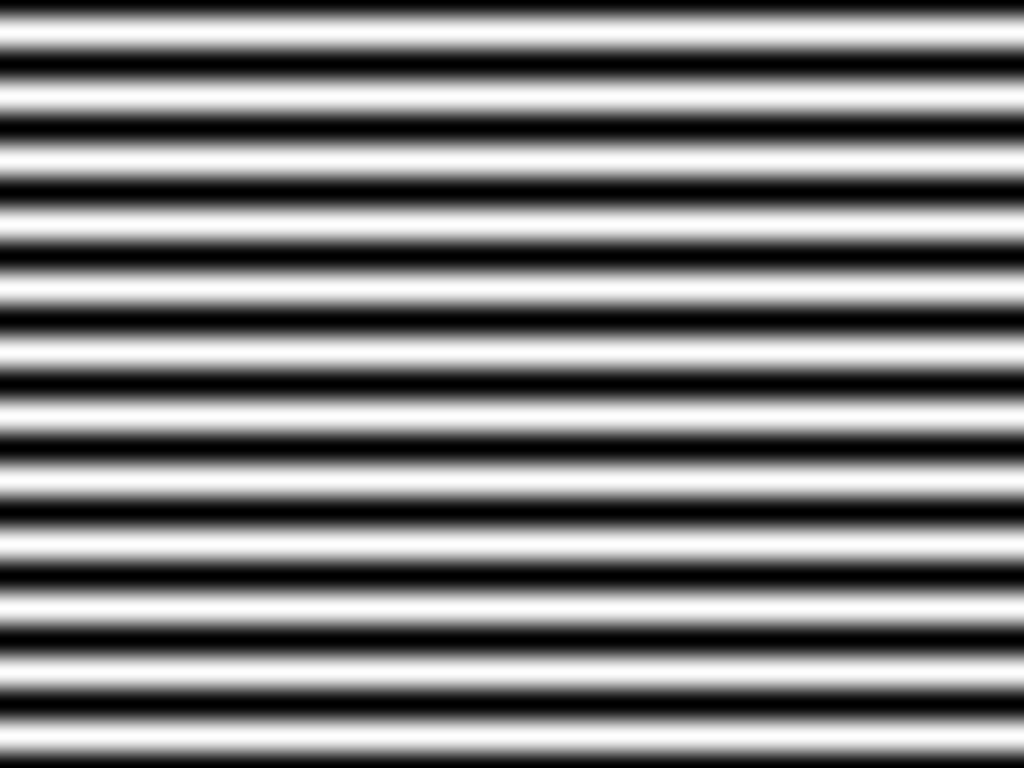
\includegraphics[width=3cm,height=3cm]{../img_source/phase_hor_1.jpg}} &
\subfloat[]{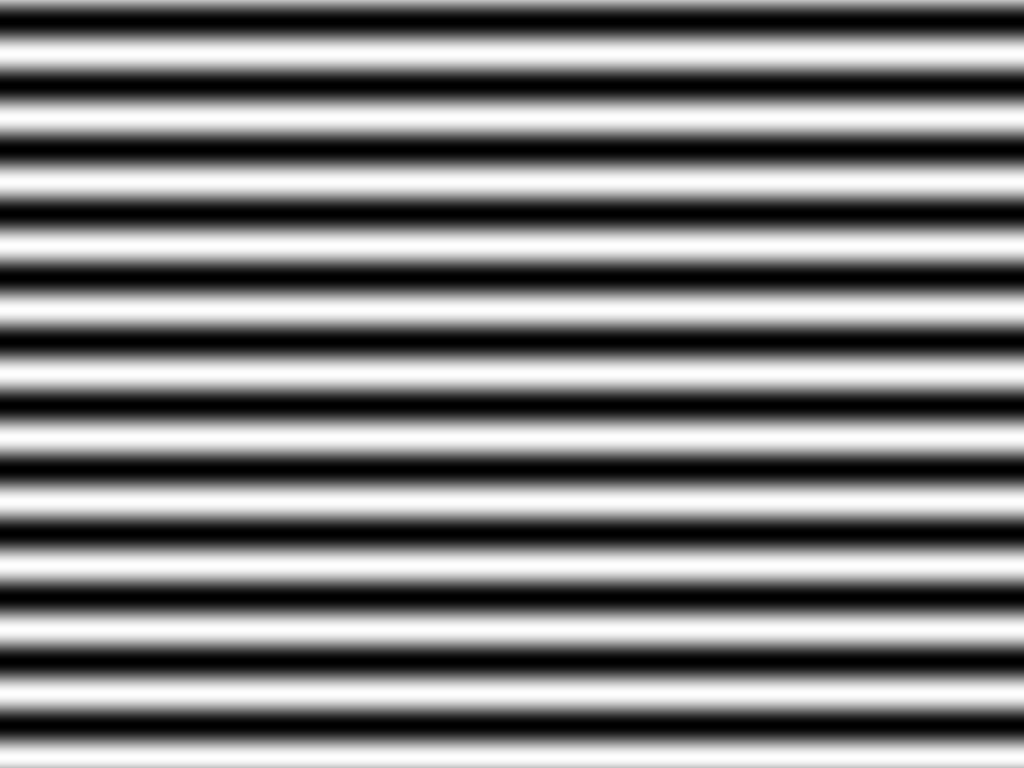
\includegraphics[width=3cm,height=3cm]{../img_source/phase_hor_2.jpg}} &
\subfloat[]{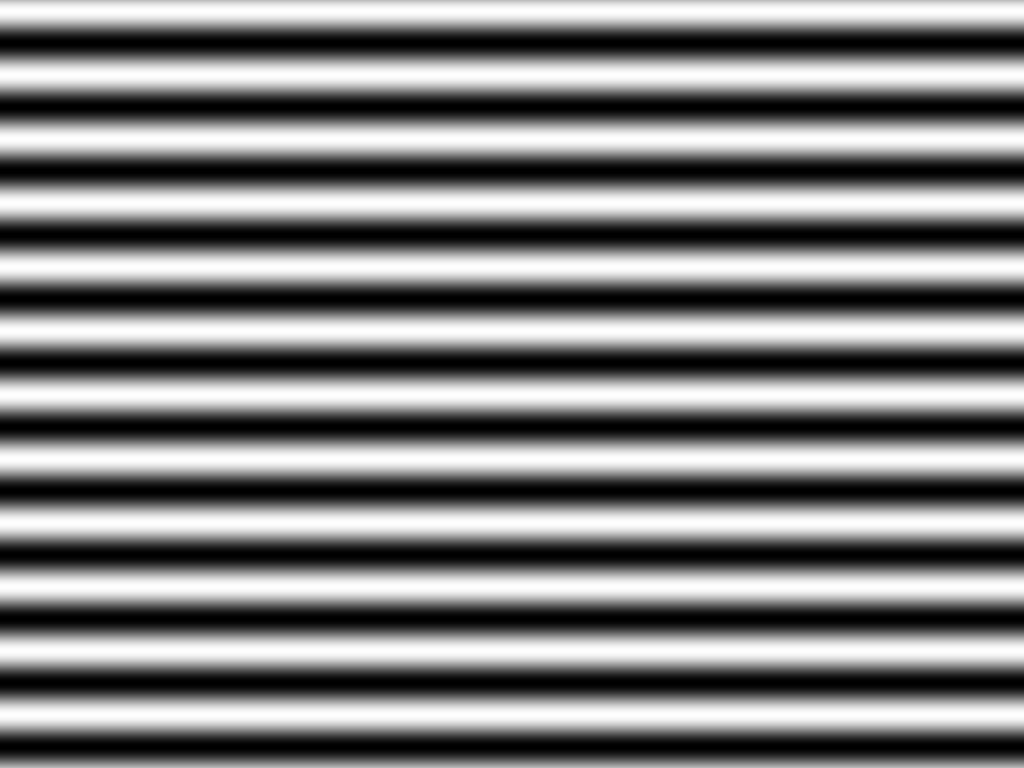
\includegraphics[width=3cm,height=3cm]{../img_source/phase_hor_3.jpg}} \\
\end{tabular}
\end{tabularx}
\caption{Horizontal phase shifted patterns}
\label{fig:hor_phase_patterns}
\end{figure}

\begin{figure}[htbp]
\centering
\def\tabularxcolumn#1{m{#1}}
\begin{tabularx}{\linewidth}{@{}cXX@{}}
\begin{tabular}{c c c}
\hspace{2.5cm}\subfloat[]{
\includegraphics[width=3cm,height=3cm]{../img_source/binary_ver_1.jpg}} &
\subfloat[]{
\includegraphics[width=3cm,height=3cm]{../img_source/binary_ver_2.jpg}} &
\subfloat[]{
\includegraphics[width=3cm,height=3cm]{../img_source/binary_ver_3.jpg}} \\
\end{tabular}
\end{tabularx}
\caption{Vertical binary coded patterns}
\label{fig:vert_bin_patterns}
\end{figure}

\begin{figure}[htbp]
\centering
\def\tabularxcolumn#1{m{#1}}
\begin{tabularx}{\linewidth}{@{}cXX@{}}
\begin{tabular}{c c c}
\hspace{2.5cm}\subfloat[]{
\includegraphics[width=3cm,height=3cm]{../img_source/binary_hor_1.jpg}} &
\subfloat[]{
\includegraphics[width=3cm,height=3cm]{../img_source/binary_hor_2.jpg}} &
\subfloat[]{
\includegraphics[width=3cm,height=3cm]{../img_source/binary_hor_3.jpg}} \\
\end{tabular}
\end{tabularx}
\caption{Horizontal binary coded patterns}
\label{fig:hor_bin_patterns}
\end{figure}


\subsection{Pattern projection and capture}
This module is developed for projection of binary coded and fringe patterns and to capture the patterns in sequential order. Currently it has only interactive control to project and capture patterns, but future version will include a synchronizing function to determine a common frequency of pattern projection and capture. In addition this module allows to control brightness of projector and camera. It allows to manipulate shutter-speed of camera hence facilitating to adapt according to varying illumination conditions. All projected and captured images are undistorted(i.e. camera/projector lens distortion effects are reduced) using the projector and camera intrinsic calibration parameters respectively. Figure~\ref{fig:capt_vert_fringe_bin} shows the captured vertical fringe and binary coded patterns. Figure~\ref{fig:capt_hor_fringe_bin} shows some captured horizontal fringe and binary coded patterns.

\begin{figure}[htbp]
\def\tabularxcolumn#1{m{#1}}
\begin{tabularx}{\linewidth}{@{}cXX@{}}
\begin{tabular}{c c c}
\hspace{1.1cm}\subfloat[]{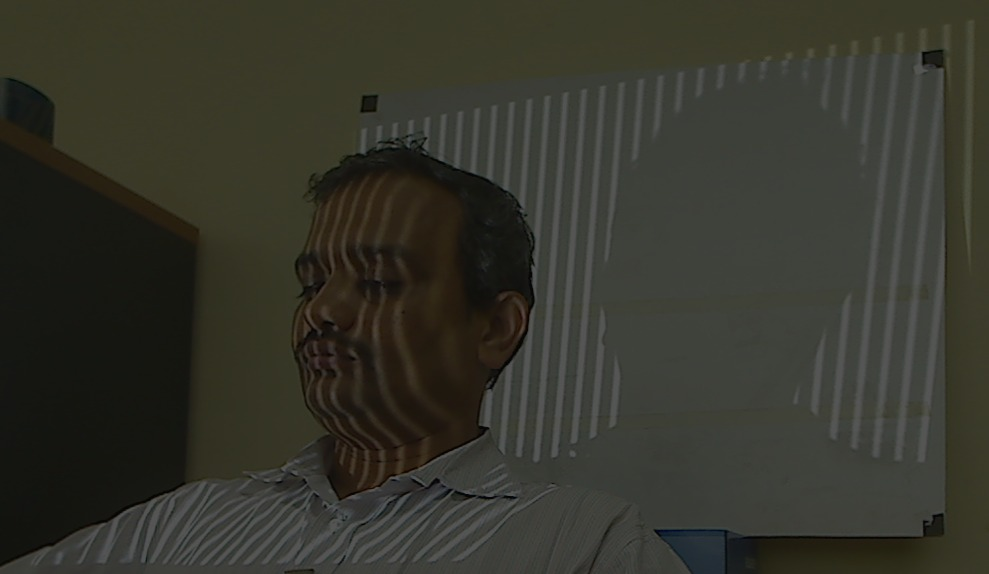
\includegraphics[width=4cm,height=4cm]{../img_source/cap_fringe_1.jpg}} &
\subfloat[]{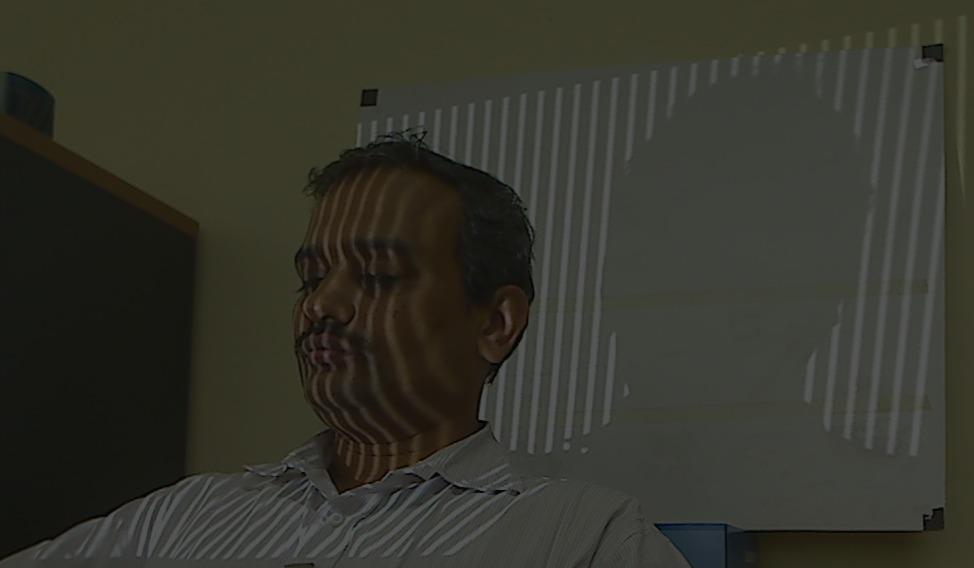
\includegraphics[width=4cm,height=4cm]{../img_source/cap_fringe_2.jpg}} &
\subfloat[]{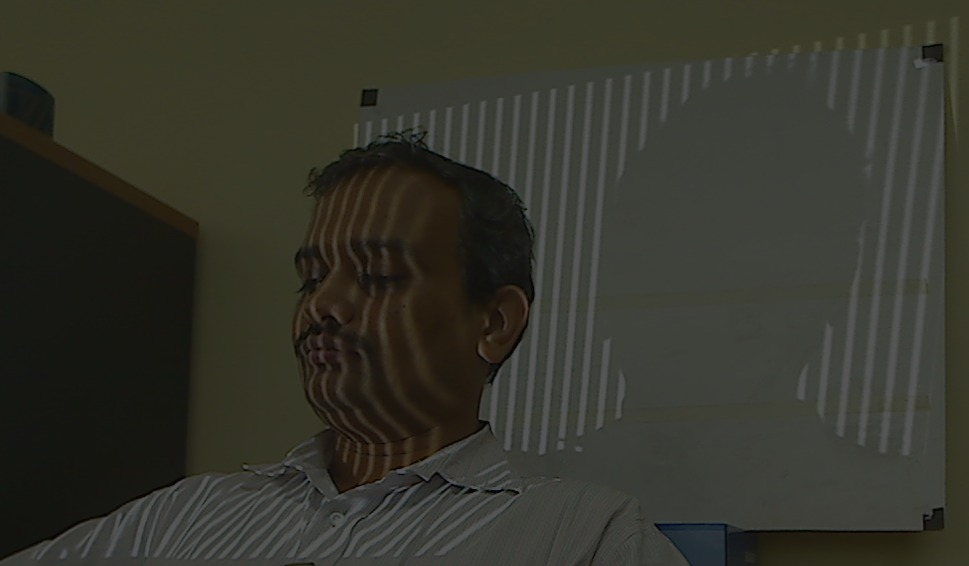
\includegraphics[width=4cm,height=4cm]{../img_source/cap_fringe_3.jpg}} \\
\hspace{1.1cm}\subfloat[]{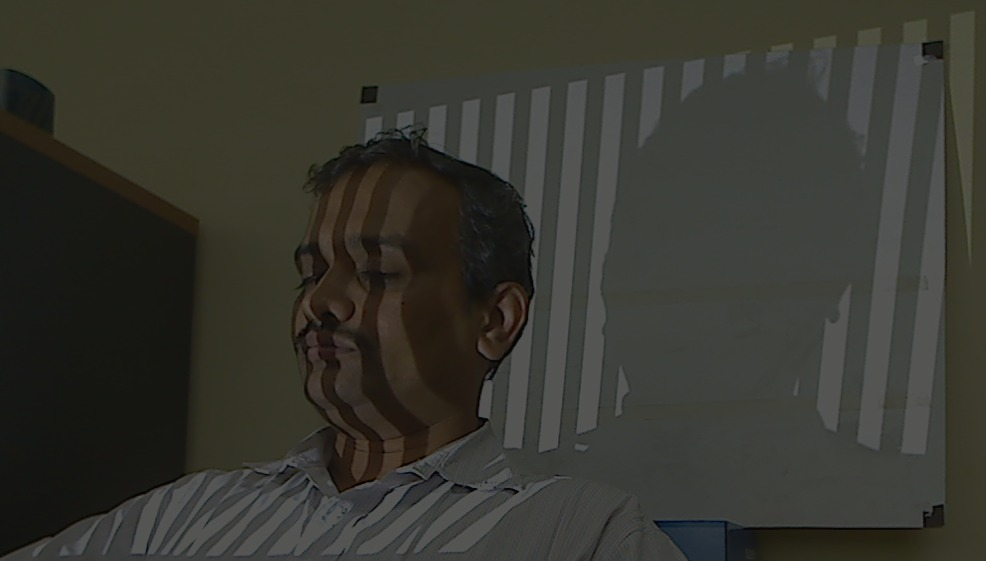
\includegraphics[width=4cm,height=4cm]{../img_source/cap_fringe_4.jpg}} &
\subfloat[]{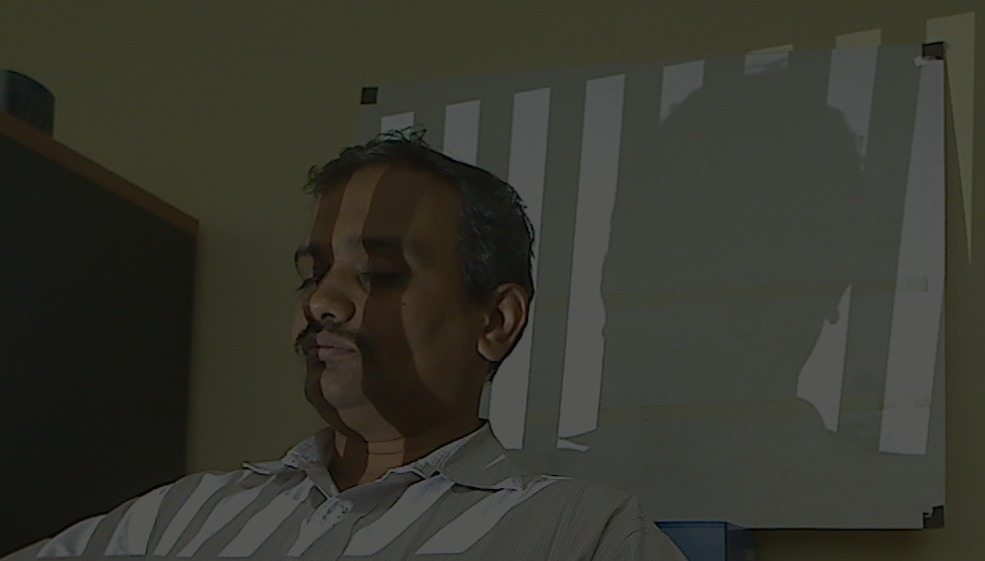
\includegraphics[width=4cm,height=4cm]{../img_source/cap_fringe_5.jpg}} &
\subfloat[]{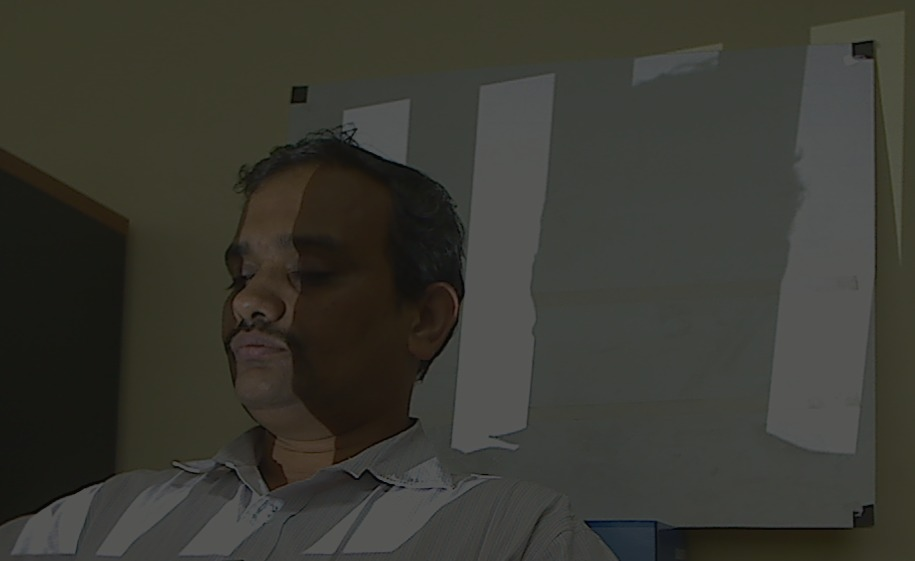
\includegraphics[width=4cm,height=4cm]{../img_source/cap_fringe_6.jpg}} \\
\end{tabular}
\end{tabularx}
\caption{Some captured vertical fringe and binary coded patterns}
\label{fig:capt_vert_fringe_bin}
\end{figure}
\begin{figure}[htbp]
\def\tabularxcolumn#1{m{#1}}
\begin{tabularx}{\linewidth}{@{}cXX@{}}
\begin{tabular}{c c c}
\hspace{1.1cm}\subfloat[]{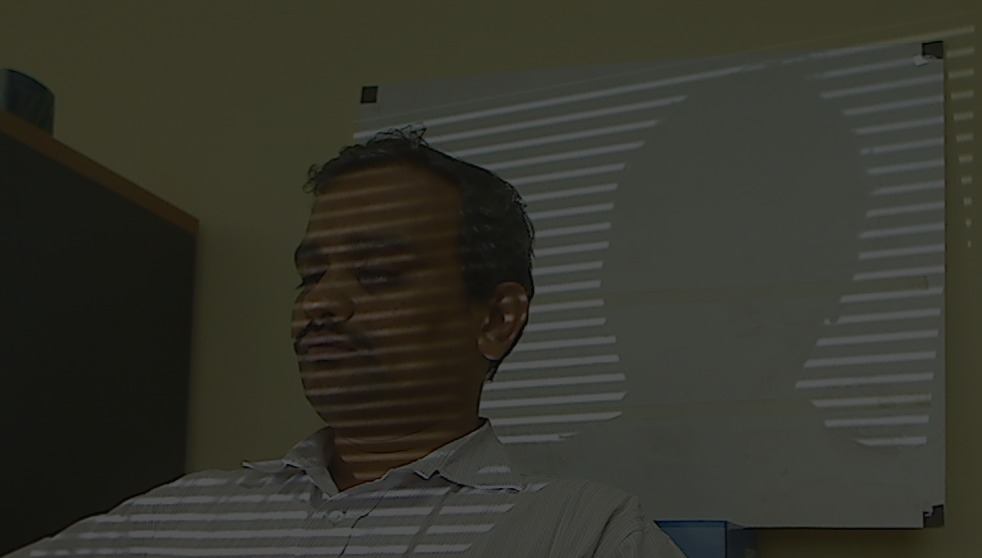
\includegraphics[width=4cm,height=4cm]{../img_source/cap_binary_1.jpg}} &
\subfloat[]{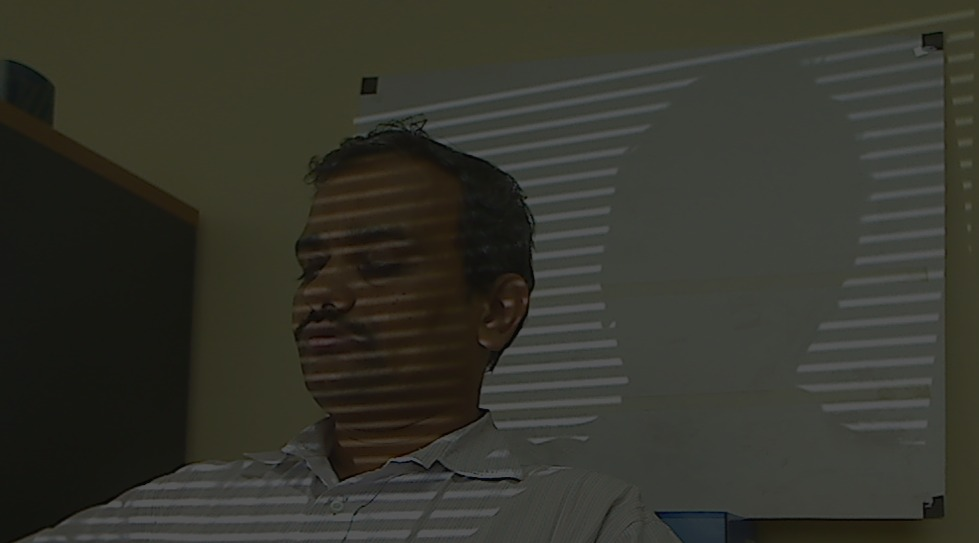
\includegraphics[width=4cm,height=4cm]{../img_source/cap_binary_2.jpg}} &
\subfloat[]{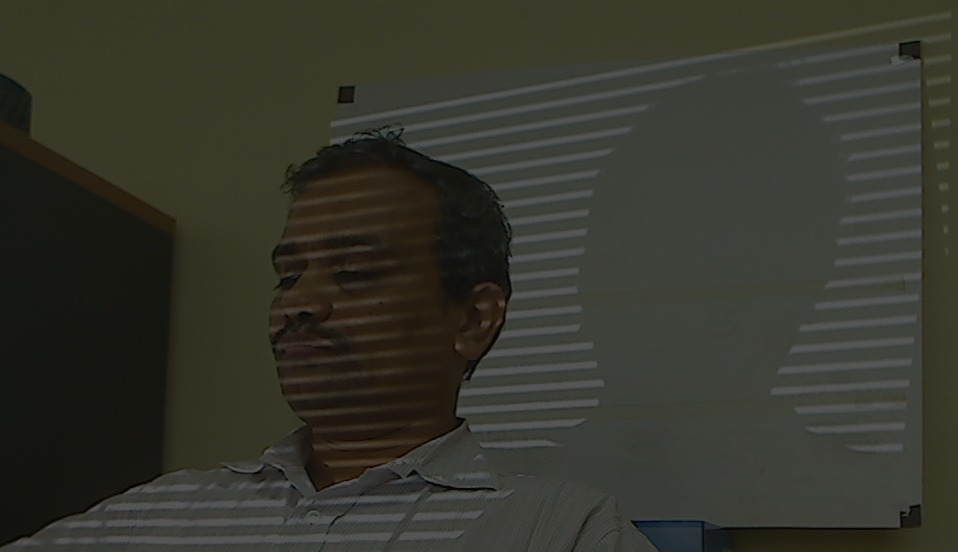
\includegraphics[width=4cm,height=4cm]{../img_source/cap_binary_3.jpg}} \\
\hspace{1.1cm}\subfloat[]{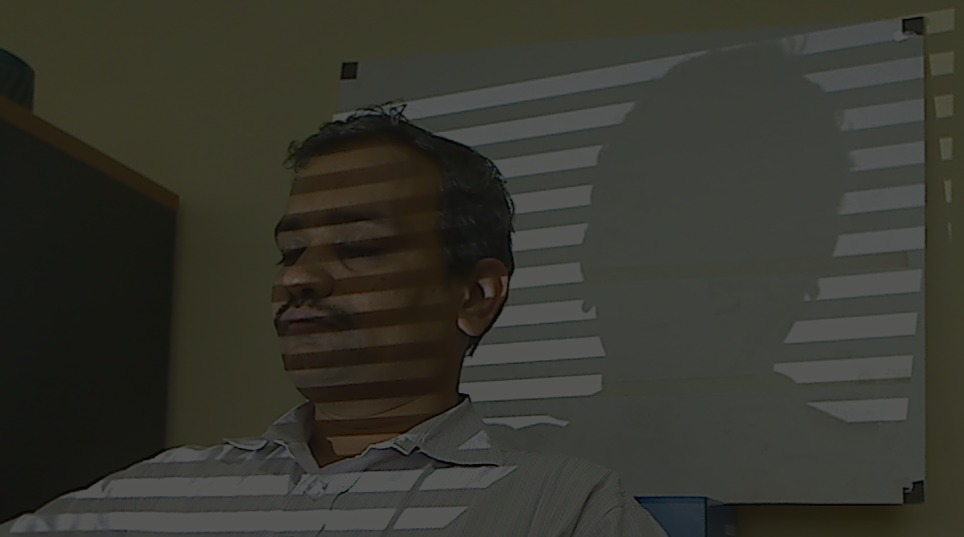
\includegraphics[width=4cm,height=4cm]{../img_source/cap_binary_4.jpg}} &
\subfloat[]{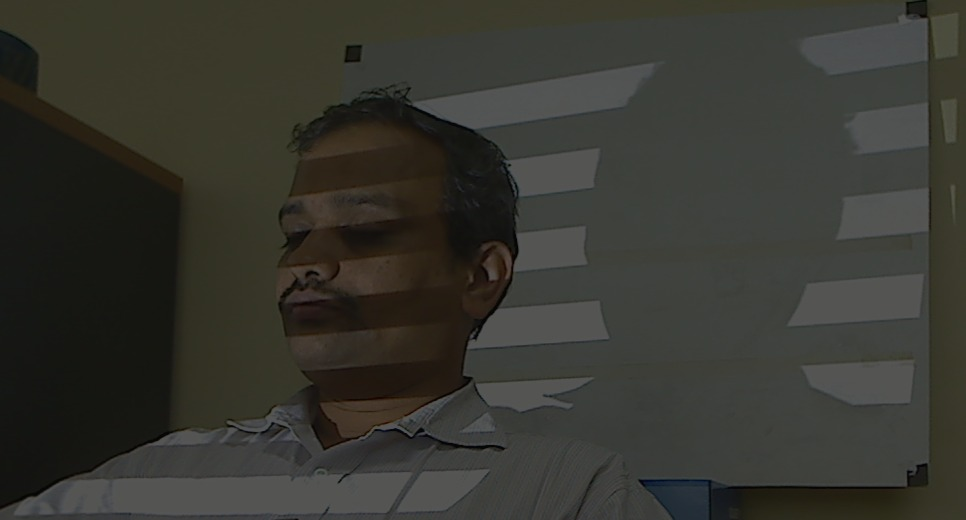
\includegraphics[width=4cm,height=4cm]{../img_source/cap_binary_5.jpg}} &
\subfloat[]{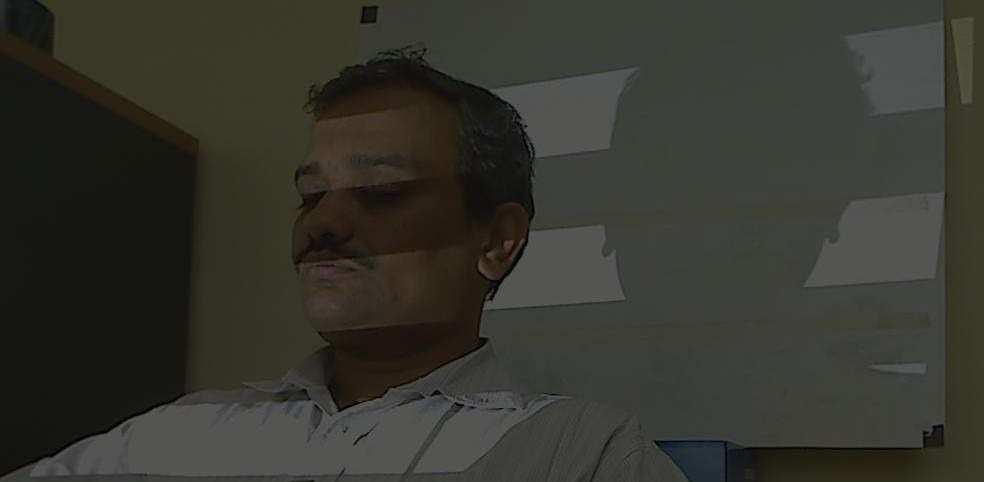
\includegraphics[width=4cm,height=4cm]{../img_source/cap_binary_6.jpg}} \\
\end{tabular}
\end{tabularx}
\caption{Some captured horizontal fringe and binary coded patterns}
\label{fig:capt_hor_fringe_bin}
\end{figure}

\subsection{Phase wrapping}
Projected sinusoidal fringe pattern is periodic in nature. It implies that there exists ambiguity in determining the phase of any point across the pattern. This ambiguity is manifested in the illumination model used in Phase-shift technique. Following equations show the assumed illumination model at every camera pixel for three phase-shift technique[9] for both horizontal and vertical fringe patterns:\newline
\begin{equation}
\begin{aligned}
& I_1=I_{dc}+I_{mod}*cos(\phi-\psi) \\
& I_2=I_{dc}+I_{mod}*cos(\phi) \\
& I_3=I_{dc}+I_{mod}*cos(\phi+\psi)
\end{aligned}
\end{equation}
\noindent
where,\newline
$I_i$: Captured intensity when $i^{th}$ pattern is projected\newline
$\phi$: Wrapped phase\newline
$\psi$: Constant phase shift between successive patterns\newline
$I_{dc}$: Background intensity\newline
$I_{mod}$: Intensity modulation\newline
\noindent
Assuming $\psi=\frac{2\pi}{3}$,using this system of equations $\phi$ can be solved at every pixel as:\newline

\begin{equation}
\phi=tan^{-1}\bigg[\frac{\sqrt[2]{3}(I_1-I_3)}{2I_2-I_1-I_3}\bigg]
\end{equation}
where, $-\pi\leq\phi\leq\pi$ \newline
\noindent
Since $\phi$ lies from $-\pi$ to $\pi$, information regarding actual phase at every point is mapped to this range hence it is called \textit{wrapped phase}. It cannot be resolved for correct corresponding projector pixel unless we compute the corresponding period number. This task is performed by module described in next subsection. Figure~\ref{fig:wrapped_phase} shows the wrapped phase computed from the captured phase shifted fringe images.

\begin{figure}[htbp]
\def\tabularxcolumn#1{m{#1}}
\begin{tabularx}{\linewidth}{@{}cXX@{}}
\begin{tabular}{c c}
\hspace{2cm}\subfloat[Vertical wrapped phase]{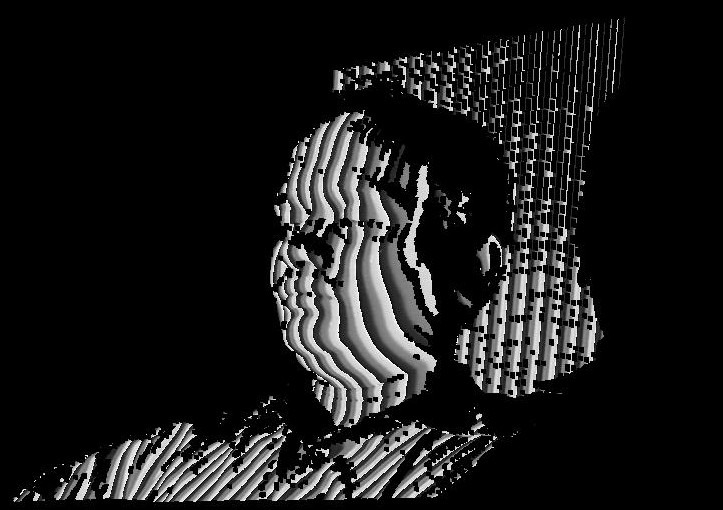
\includegraphics[width=4.5cm,height=4cm]{../img_source/wrapped_ver.jpg}} &
\hspace{2cm}\subfloat[Horizontal wrapped phase]{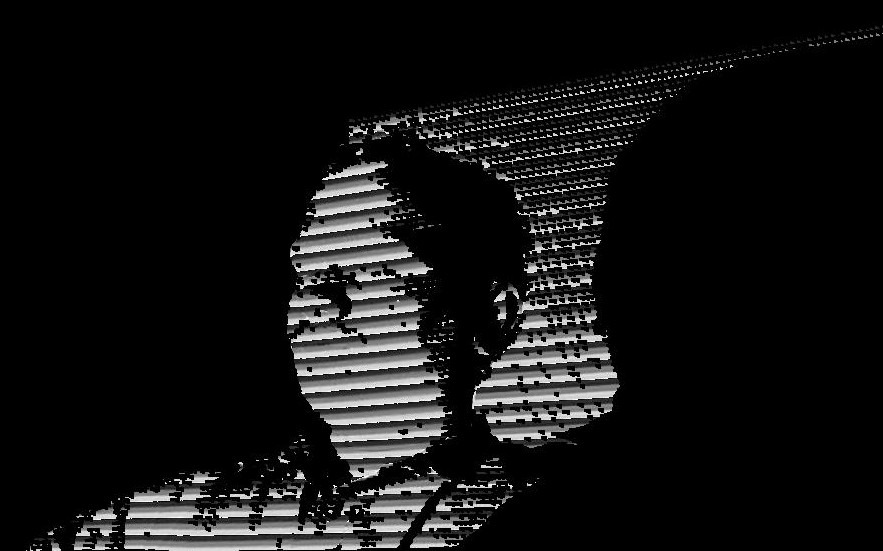
\includegraphics[width=4.5cm,height=4cm]{../img_source/wrapped_hor.jpg}}\\
\end{tabular}
\end{tabularx}
\caption{Computed wrapped phase}
\label{fig:wrapped_phase}
\end{figure}

\paragraph{Extension to four and five phase shifted fringe patterns.}
In order to assess the effect of increasing the number of phase shifted patterns on accuracy of estimated stereo-correspondence,  the basic 3D scanner with 3 phase shifted patterns was extended to be able to project and process four and five phase shifted patterns also. It should be noted however that only pattern generator and phase wrapper modules need to be extended for this purpose as all remaining modules are independent of number of patterns used for 3D scanning. Further it should be pointed out that \textit{three} is the minimum number of phase shifted patterns that can be used assuming $I_{dc}$, $I_{mod}$ and $\phi$ as unknowns which requires at least 3 equations and hence 3 patterns. Equation 3-7 describes assumed illumination model for 4 phase-shifted pattern technique,  equation 3-8 expresses the corresponding wrapped phase. Whereas equation 3-9 expresses the illumination model for 5 phase shifted pattern technique and equation 3-10 represents the corresponding wrapped phase. Unknowns $I_{dc}$, $I_{mod}$, $\phi$ have same meaning as in equation 3-5,3-6.\newline
\noindent
For four sinusoidal fringe patterns phase-shifted by $\pi/2$,
\begin{equation}
\begin{aligned}
& I_0=I_{dc}+I_{mod}*cos(\phi) \\
& I_1=I_{dc}+I_{mod}*cos(\phi+\pi/2) \\
& I_2=I_{dc}+I_{mod}*cos(\phi+\pi) \\
& I_3=I_{dc}+I_{mod}*cos(\phi+3\pi/2)
\end{aligned}
\end{equation}
Simultaneously solving equations 3-7 gives wrapped phase, $\phi$ as:
\begin{equation}
\phi=tan^{-1}\bigg[\frac{I_3-I_1}{I_0-I_2}\bigg]
\end{equation}
Similarly for five sinusoidal fringe patterns phase-shifted by $2\pi/5$,
\begin{equation}
\begin{aligned}
& I_0=I_{dc}+I_{mod}*cos(\phi-4\pi/5) \\
& I_1=I_{dc}+I_{mod}*cos(\phi-2\pi/5) \\
& I_2=I_{dc}+I_{mod}*cos(\phi) \\
& I_3=I_{dc}+I_{mod}*cos(\phi+2\pi/5)\\
& I_4=I_{dc}+I_{mod}*cos(\phi+4\pi/5)
\end{aligned}
\end{equation}
Solving equations 3-9 gives wrapped phase $\phi$ as: 
\begin{equation}
\phi=tan^{-1}\bigg[2sin\alpha*\bigg(\frac{I_1-I_3}{2I_2-I_4-I_0}\bigg)\bigg]
\end{equation}


\subsection{Pixel decoding and phase unwrapping}
Periodic nature of sinusoidal interference fringes creates ambiguous condition in which multiple pixels in camera image can have same wrapped phase hence there is need to assign distinct period numbers to such candidates thereby eliminating the ambiguity. This step is called \textit{phase unwrapping}. Therefore a module to perform phase unwrapping was developed which uses information from binary code projected onto the object to recover this period number. It should be noted here that wrapped and hence unwrapped phase is computed in both vertical and horizontal directions. Hence we get a pair of unwrapped phase associated with each valid camera pixel. Here a camera pixel is called \textit{valid} if it corresponds to the region on which pattern is projected and has a Signal/Noise ratio greater than a threshold(this threshold is environment illumination dependent in current implementation).Equation 3.11 describes the criteria used as a measure of Signal/Noise ratio for 3 phase-shift approach.
\begin{equation}
\eta=\frac{I_{mod}}{I_{dc}}=\frac{\sqrt[2]{3(I_1-I_3)^2+(2I_2-I_1-I_3)^2}}{I_1+I_2+I_3}
\end{equation}
Here,$\eta$ represents the Signal/Noise ratio,hence,pixel(x,y) is \textit{valid} if $\eta(x,y)>T$,where $T$ is assumed threshold.


Unwrapped phase is calculated using information from both fringe projection and binary coded techniques as. Following equation represent represents this problem:\newline

\begin{equation}
\oint(x,y)=\phi(x,y)+2\pi*C(x,y)
\end{equation}
\noindent
where,\newline
$\oint(x,y)$: Unwrapped phase at pixel (x,y)\newline
C(x,y): Decoded binary code at pixel (x,y)\newline
\noindent
This equation is applied for both horizontal and vertical phase unwrapping. Figure~\ref{fig:unwrapped_phase} represents the unwrapped phase corresponding to the wrapped phase shown in figure~\ref{fig:wrapped_phase}.

\begin{figure}[ht]
\def\tabularxcolumn#1{m{#1}}
\begin{tabularx}{\linewidth}{@{}cXX@{}}
\begin{tabular}{l r}
\hspace{2cm}\subfloat[Vertical unwrapped phase]{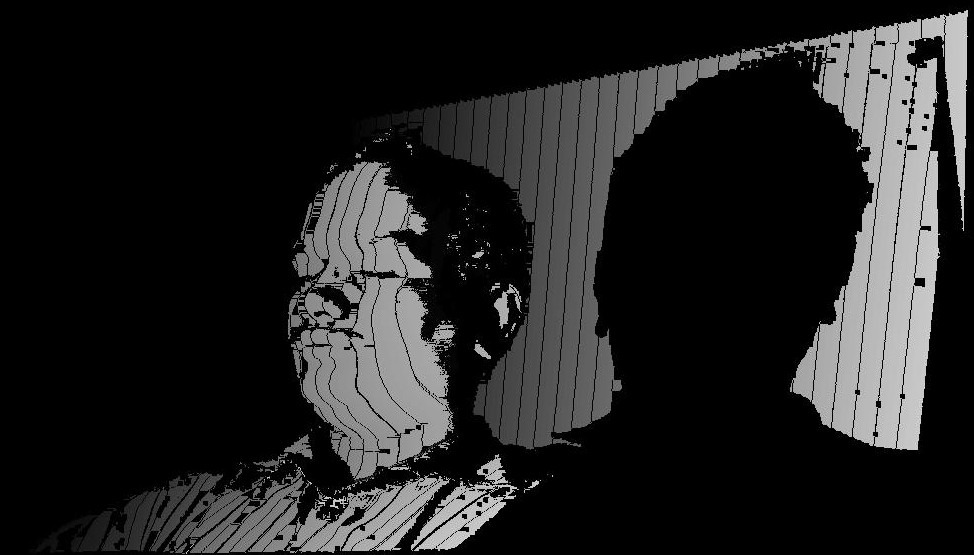
\includegraphics[width=4.5cm,height=4cm]{../img_source/unwrapped_ver.jpg}} &
\hspace{2cm}\subfloat[Horizontal unwrapped phase]{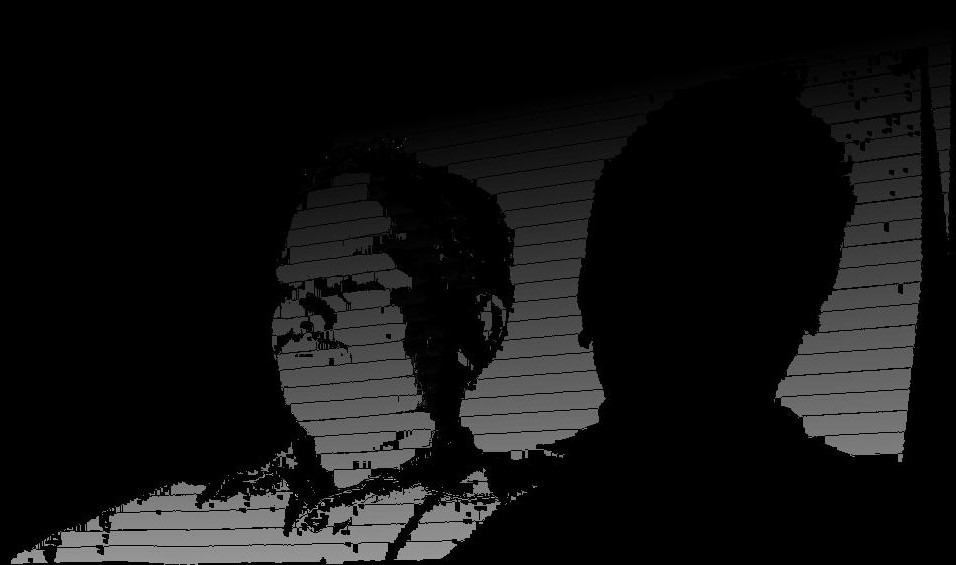
\includegraphics[width=4.5cm,height=4cm]{../img_source/unwrapped_hor.jpg}}\\
\end{tabular}
\end{tabularx}
\caption{Computed unwrapped phase}
\label{fig:unwrapped_phase}
\end{figure}

\subsection{Correspondence computation using absolute phase}
Stereo-correspondence between binocular elements like a projector-camera pair relates the points in projector and camera image-space which are observing a common 3D point in the scene.\newline% Figure~\ref{fig:correspond_abstract} shows stereo-correspondence for clarity. Here a point in left view is related to a point in right view because they are 2D projections of a common point named \textit{Scene Point} in the scene using estimated stereo-correspondence.
%\begin{figure}
%\centering
%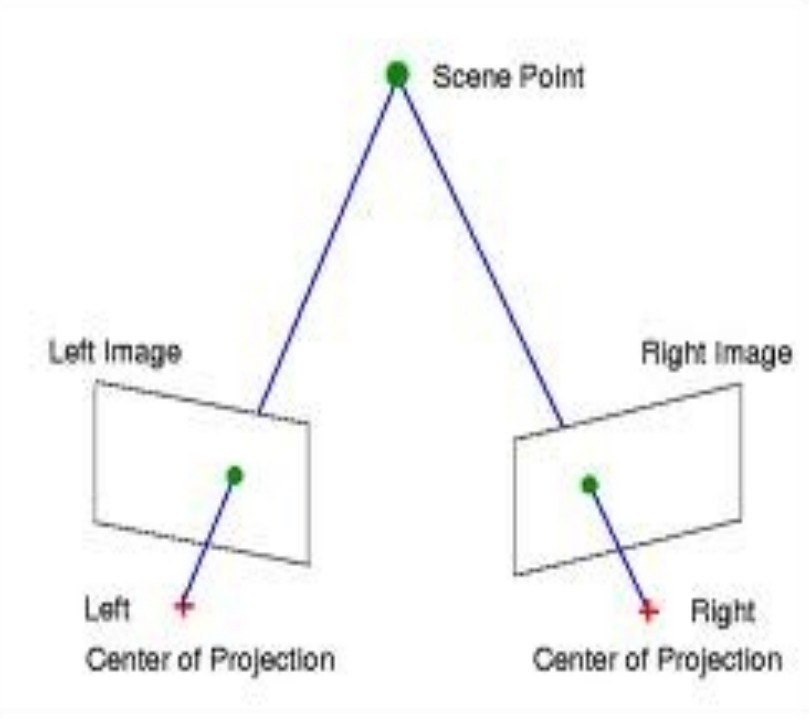
\includegraphics[width=8cm,height=8cm]{../img_source/stereo_correspondence_abstract.jpg}
%\caption{Stereo correspondence:abstract representation}
%\label{fig:correspond_abstract}
%\end{figure}
%\begin{figure}
%\begin{tikzpicture}
%\fill[green] (0,0) circle[radius=2pt];
%\draw (-3,) rectangle ();
%\end{tikzpicture}
%\end{figure}
%\noindent
\indent Once the unwrapped phase is computed,camera-projector pixel-pixel correspondences can be computed directly by searching for pixels in projector with same vertical and horizontal unwrapped phase values as that of corresponding valid camera pixel. It is computed as:
\begin{equation}
\begin{aligned}
& X_p=\lfloor w_{fringe}*\big(\frac{\oint_v(X_c,Y_c)}{2\pi}\big) \rfloor \\ 
& Y_p=\lfloor w_{fringe}*\big(\frac{\oint_h(X_c,Y_c)}{2\pi}\big) \rfloor
\end{aligned}
\end{equation}
\noindent
where,\newline
$(X_p,Y_p)$: Projector coordinates corresponding to camera coordinates $(X_c,Y_c)$\newline
$w_{fringe}$: Width of projected fringe in pixels.\newline
Figure~\ref{fig:estimated_correspondence} shows the one result of correspondence computation using the developed system.
\begin{figure}[htbp]
\def\tabularxcolumn#1{m{#1}}
\begin{tabularx}{\linewidth}{@{}cXX@{}}
\begin{tabular}{c c}
\hspace{2cm}
\subfloat[Camera image]{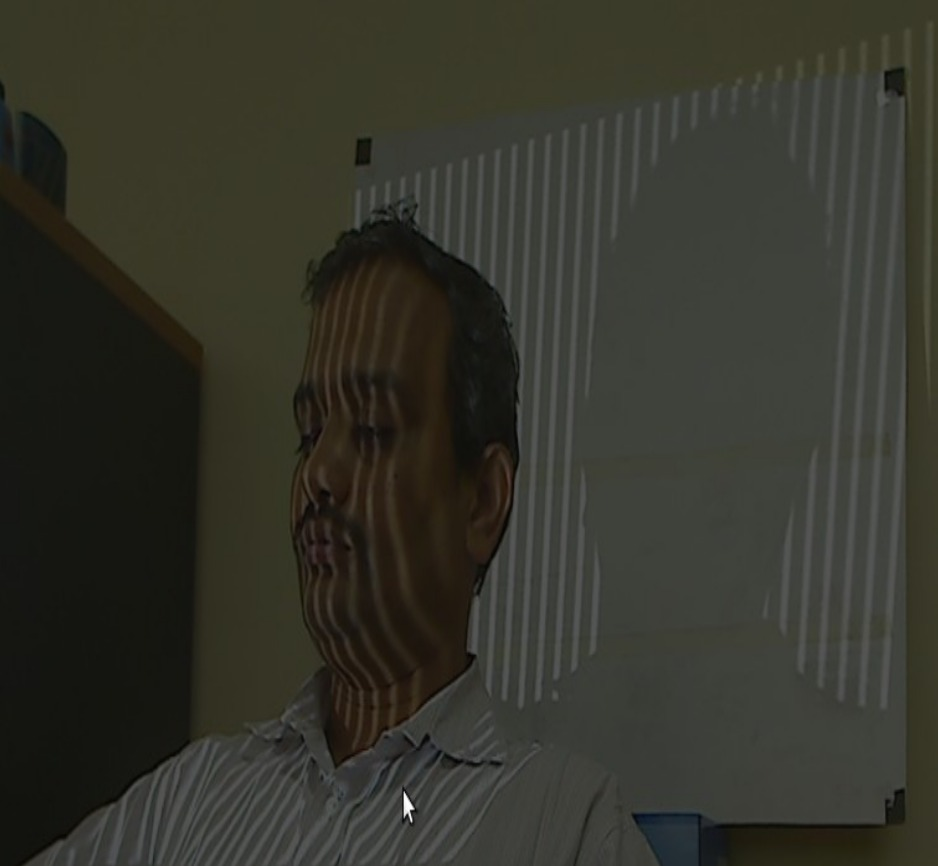
\includegraphics[width=4.5cm,height=4cm]{../img_source/camera_image.jpg}} &
\hspace{2cm}\subfloat[Projector image]{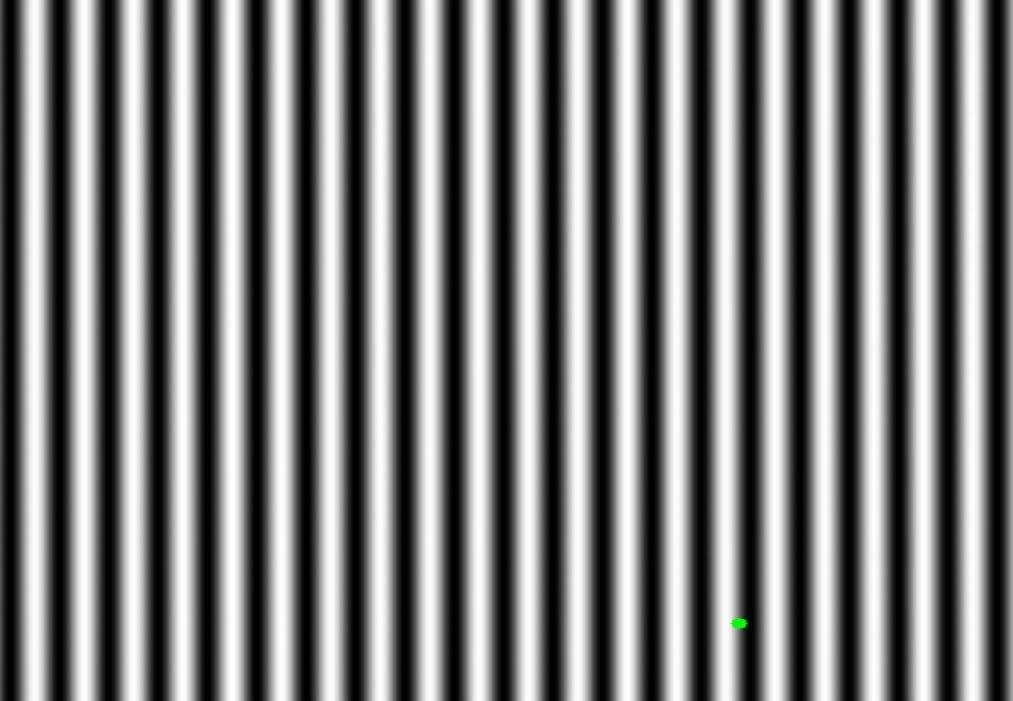
\includegraphics[width=4.5cm,height=4cm]{../img_source/projector_image.jpg}} 
\end{tabular}
\end{tabularx}
\caption{Stereo correspondence between camera and projector:\textit{green} spot in (b) corresponds to selected point(cursor) in (a)}
\label{fig:estimated_correspondence}
\end{figure}




\section{Discussion}
It was observed that phase-shift technique do not work well on surface with very high(or very low) surface reflectance, surface interreflections, subsurface scattering and in cases when projector or camera is/are defocused. These problems are still a limitation of structured light technique. However some developments for this problem have been reported recently[46].\newline
\indent Further, an ambiguity in decoding the binary coded patterns was observed at the edges of strips which due to projector or camera blur becomes wider \textit{grey} region which cannot be reliably judged black or white in general. Because of this problem, points in the strip region were discarded while evaluating accuracy and precision of the system.\newline
\indent Although original plan was to fully develop the system purely based on phase-shift technique but our phase-unwrapping implementation[47] was not converging to a solution and was running for >3hrs without solution(on Core2Duo processor E8400 at 3.0GHZ and 2 GB RAM) for an image resolution of 960X720 even after several attempts to check correctness of implementation hence keeping project deadline and time-efficiency of the solution to be developed under consideration it was decided to shift to a combination phase-shift and binary-coded technique to reduce the computation time requirement in the phase-unwrapping process


\section{Summary}
In this chapter, the taxonomy of state-of-art approaches for 3D metrology was presented. Since this work is concerned with structured-light based techniques, a brief review of currently used approaches in this field was presented. All stages of coded phase-shift technique for estimating stereo-correspondence were described along with formal description in form of equations and real examples of output from each stage. Section 3.5 described the issues faced during development of this module. 
